\chapter{PCB 2.0 设计和测试}
\label{cha:PCB-v2}

本章设计源文件和历史版本详见\url{https://github.com/TingliangZhang/Misaka-PCB-v2}

\section{需要解决的问题}

在测试版本的PCB(PCB v1)中出现了不少经过测试发现的问题,在第二版本中尽可能予以纠正:

\begin{itemize}
    \item ATmega2560的晶振封装无法手焊,而且不在嘉立创基础库里,不方便SMT
    \item PowerSTEP01过于昂贵,而且极难手动贴片。
\end{itemize}

\section{设计环境的更改}

PCB的设计依赖电子设计自动化(英语:Electronic design automation,缩写:EDA)软件。

当初绘制PCB v1时使用的时Altium Designer 20.0.9集成开发环境。

由于AD20是商业付费EDA软件,而且之前的绘制使用了Altium Live 在线供应商封装库,可移植性和便携性不是很好,即使生成了Integrated Library,也很难找到成套的规范化封装。另外AD20的源文件不是普通编辑器可以打开的文本,这使得Git代码管理变得困难。

基于以上考量,改用KiCAD开源EDA软件进行目前及将来的电路设计,如图~\ref{fig:kicad_flowchart}。

\begin{figure}[htbp]
    \centering
    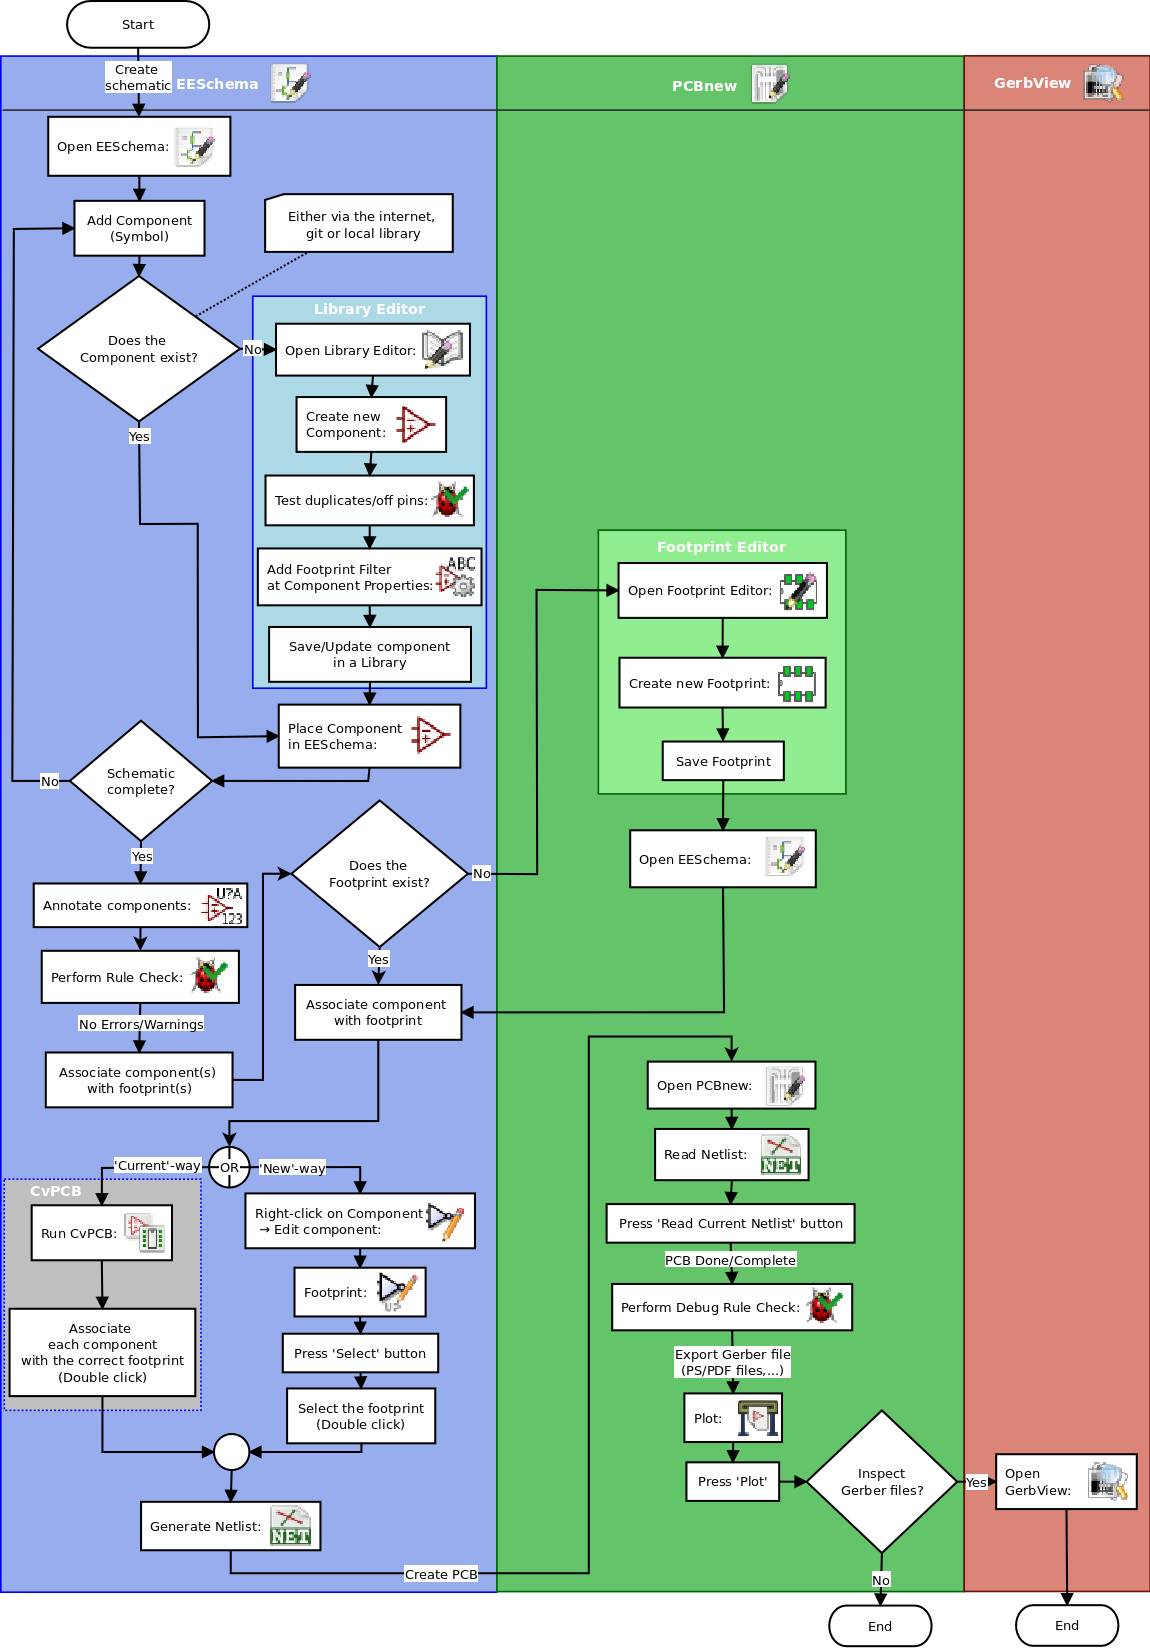
\includegraphics[width=\columnwidth]{kicad_flowchart.png}
    \caption{KiCad Workflow}
    \label{fig:kicad_flowchart}
\end{figure}